\chapter{Introduction}\label{introduction}
The effective control of an inverted pendulum is still an active area of research nowadays. \cite{JHuber}

One type of this kind of systems is a setup called Cubli. It consists of a cube controlled with reaction wheels. The Cubli can jump up and balance on one of its edges or on one of its corners, as shown in \figref{CubliCorner}.
The Cubli is designed as a simple setup to let control engineers work with an inverted pendulum. A working Cubli can also be an interesting way to show and explain the general public  what control engineering is about. \cite{MGajamohan}
%
\begin{figure}[H] 
	\centering
	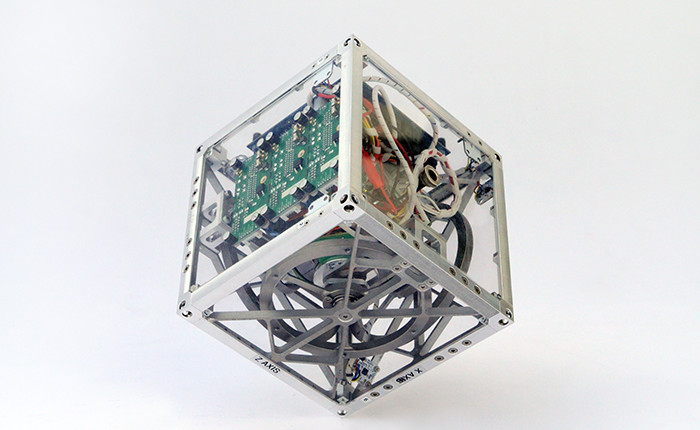
\includegraphics[scale=1.3]{figures/CubliCorner-700x430}
	\caption{A Cubli balancing on one of its corners\cite{RAndrea}}
	\label{CubliCorner}
\end{figure}
%
Applications for this cube robot, that moves without any external tools, might seem limited when you only have a single cube. However, if you take a group of cubes, they could move together to traverse obstacles or solve puzzles one cube alone could not. A group of cubes can form a structure (\figref{MBlocksExample}), and by talking in between each other they can use their reaction wheels to get the structure to move in the desired direction. Since each cube can move independently, a single cube can detach for an assignment or catch up with the main structure if it gets dropped. \cite{JRomanishin}
%
\begin{figure}[H] 
	\centering
	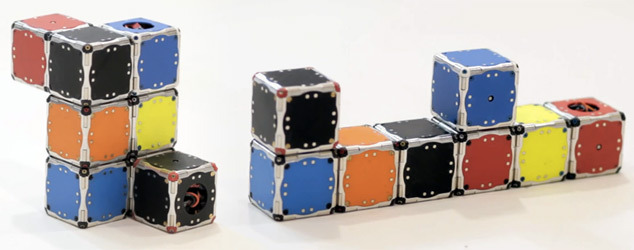
\includegraphics[scale=0.4]{figures/m-blocks}
	\caption{A number of cube robots (called M-blocks at Massachusetts Institute of Technology (MIT)) shown making two different structures. These M-blocks stick together with the help of magnets placed in their corners \cite{LRosen}}
	\label{MBlocksExample}
\end{figure}
%
It has also been suggested using similar technology for alternative locomotion in planetary or asteroid exploration. The internal actuation is not very efficient in high gravity environments, however, in environments with microgravity such as asteroids the technology becomes very feasible. \cite{RAllen}

In microgravity a Cubli could tumble or even jump across the surface. A traditional rover with wheels would not be able to sufficiently grip or might even push the rover off the surface long enough for it to land upside down. Where such a situation would be fatal for most rovers, a cube with internal actuation would not be immobilized by landing upside down.\cite{ELandau}

This concept was the basis of a small experimental lander called MINERVA, short for Micro/Nano Experimental Robot Vehicle for Asteroids, which were to explore the near earth asteroid Itokawa (see \figref{MINERVA}). The lander was deployed from its mother spacecraft HAYABUSA in 2005, when it unfortunately missed the asteroid's small gravitational pull and drifted off into space. \cite{TYoshimitsu}
%
\begin{figure}[H] 
	\centering
	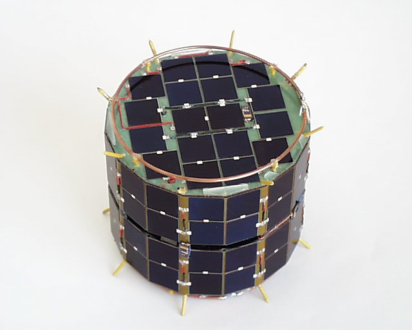
\includegraphics[scale=.8]{figures/MINERVA}
	\caption{MINERVA experimental lander, which was designed for asteroid exploration \cite{TYoshimitsu}}
	\label{MINERVA}
\end{figure}
%
A more recent example of development in this area is NASA's Hedgehog robot, which also is actuated internally with reaction wheels. It has bee through several tests aboard an aircraft for microgravity research in June 2015, where it showed its ability to jumping out of a sandpit. A picture of the Hedgehog robot can be seen in \figref{Hedgehog}. \cite{ELandau}
%
\begin{figure}[H] 
	\centering
	\includegraphics[scale=0.05]{figures/Hedgehog}
	\caption{NASA's Hedgehog robot for asteroid exploration \cite{ELandau}}
	\label{Hedgehog}
\end{figure}
%
